While text-only pre-trained models achieves great success on various NLP tasks, we live in a multimodal world and human brains naturally learn to process multi-sense signals received from the environment to help us make sense of the world around us~\citep{gan2022vision}. Among multiple modalities, vision and language are two main channels with which humans perceive and communicate, respectively. Therefore, Vision-and-Language (VL) has been a popular research area that sits at the nexus of Computer Vision and Natural Language Processing (NLP), aiming to develop algorithms that endow computers with an ability to effectively learn from multimodal data. Inspired by the great success of LLM pre-training in NLP, which is described in previous chapters, Vision-Language Pre-training (VLP) has attracted rapidly growing attention from both CV and NLP communities and become the main paradigm for modern VL research. 

In this section, we first 
introduce important vision and language tasks in section \ref{sec3:vl-tasks} and then present popular model architectures and pre-training objectives for vision-language models (VLMs) in \Cref{sec3:vl-tasks}.
% and section \ref{}, respectively. 

\section{Vision-and-Language Tasks}
\label{sec3:vl-tasks}
Vision-and-language tasks, by definition, should include both vision and language modalities in their inputs and outputs. According to \citet{gan2022vision}, VL tasks can be grouped into three categories: \textbf{Image-Text Tasks}, \textbf{CV Tasks as VL Tasks}, and \textbf{Video-Text Tasks}.

\begin{figure}
    \centering
    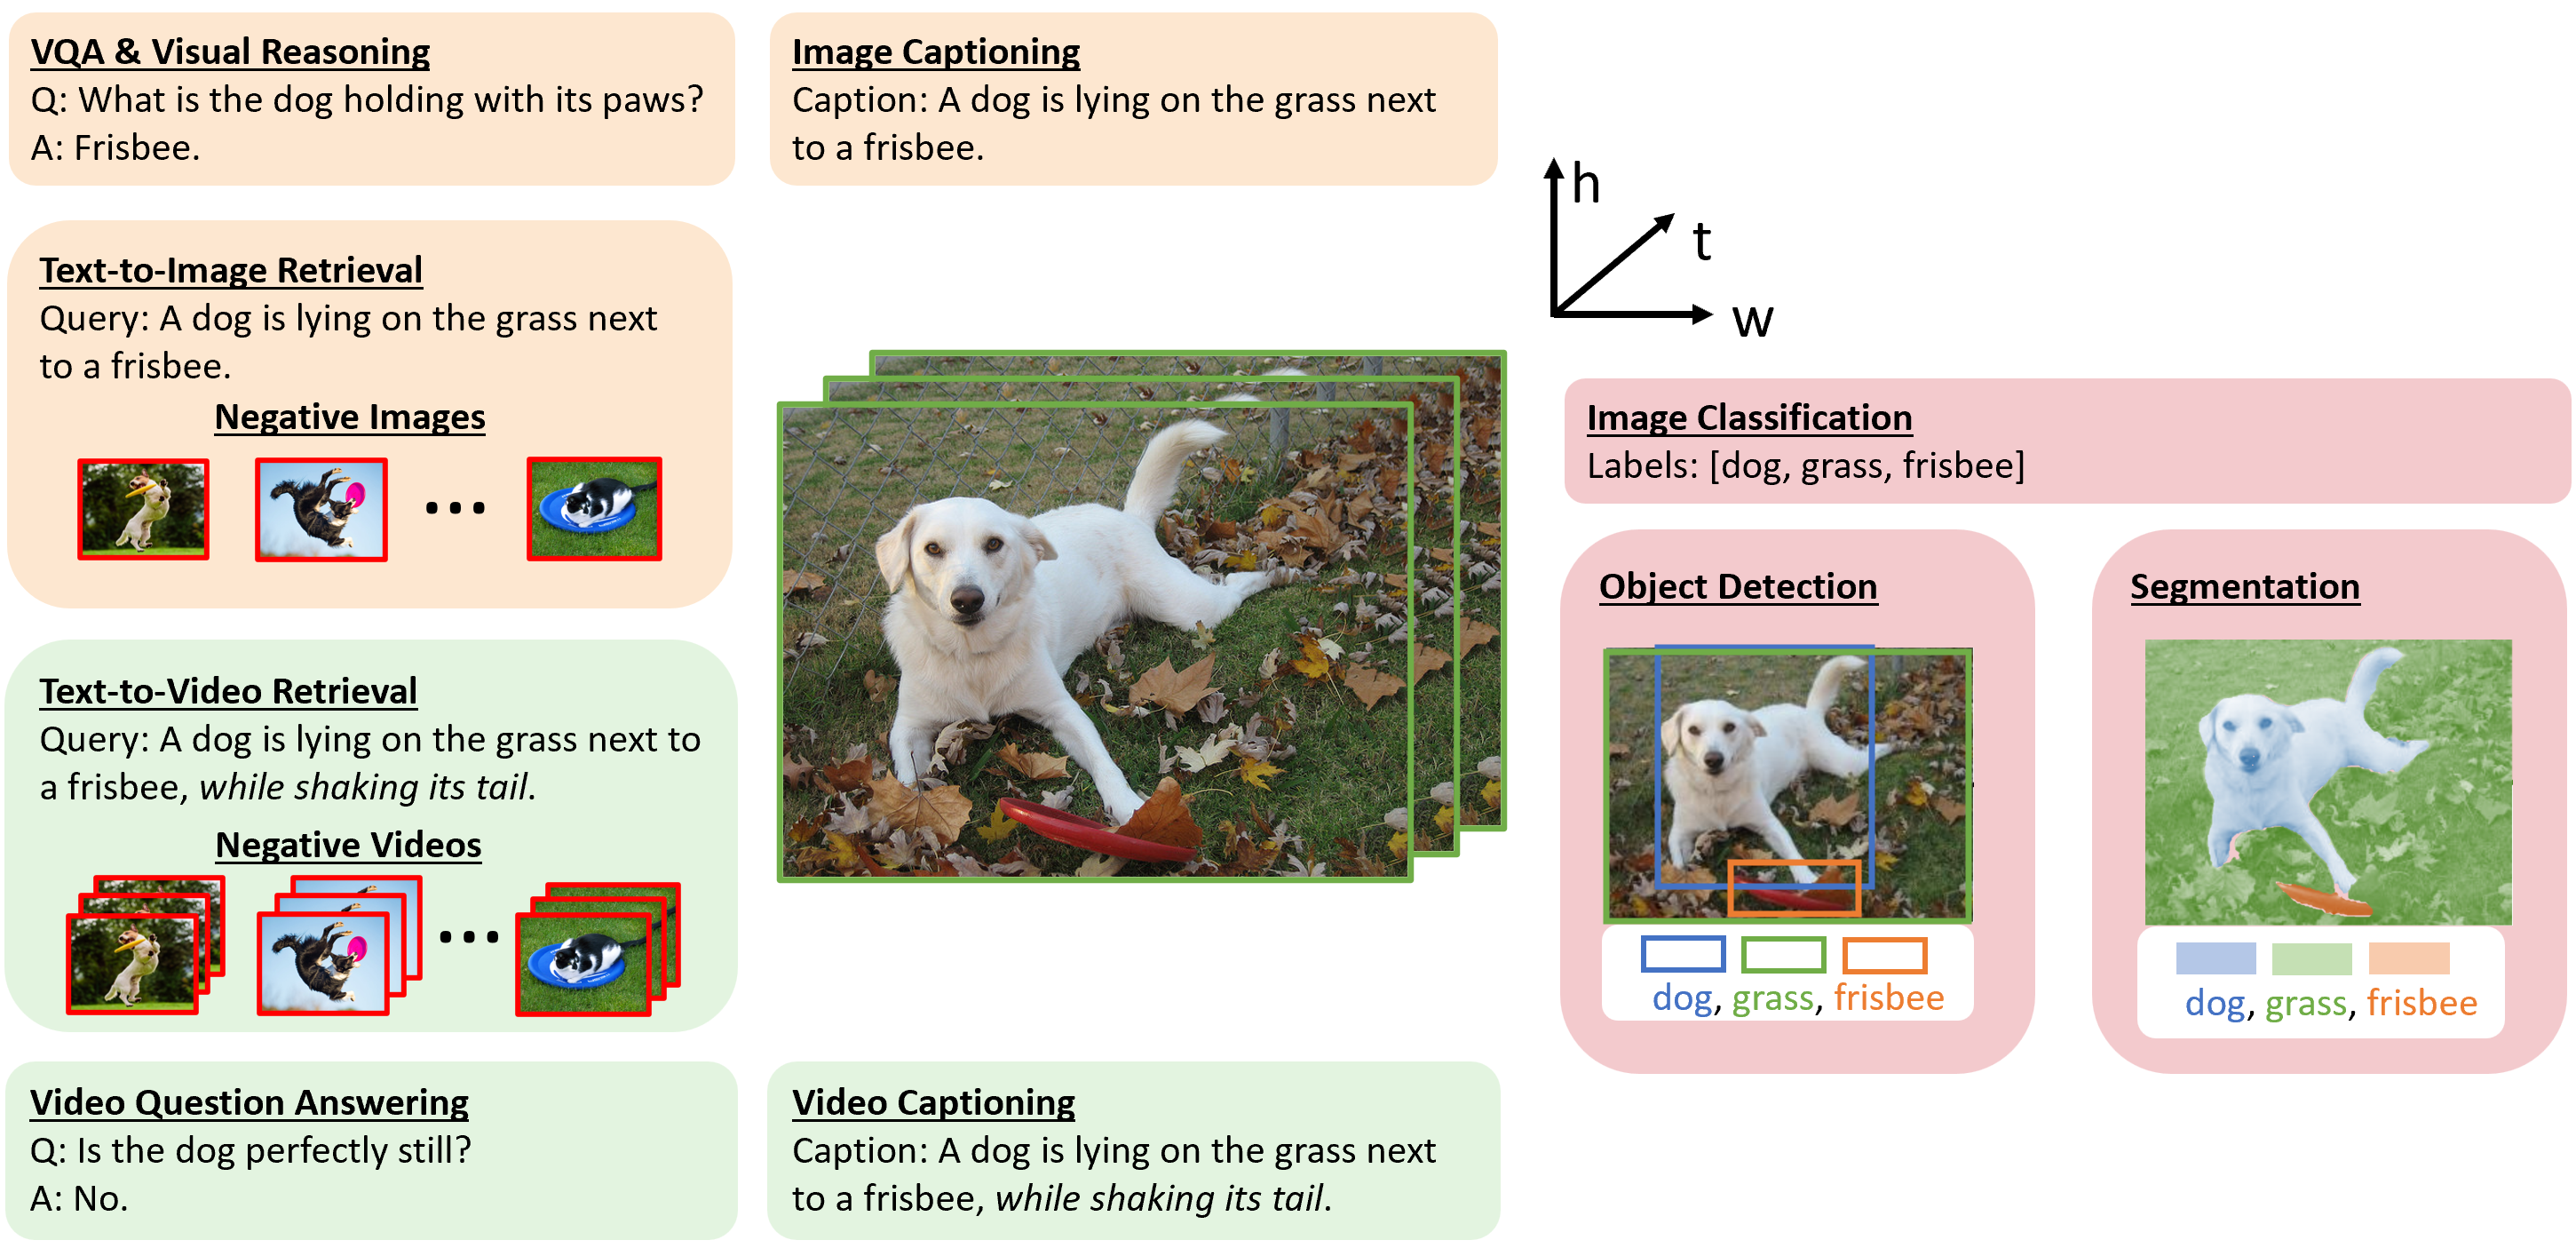
\includegraphics[width=\textwidth]{figures/multimodality/tasks.png}
    \caption{Illustration of representative tasks from three categories of VL problems covered in this paper:  \colorbox{orange!15}{image-text tasks}, \colorbox{red!15}{vision tasks as VL problems}, and \colorbox{green!15}{video-text tasks}.}
    \label{fig:chp3-vltasks}
\end{figure}

\paragraph{Image-Text Tasks.} Image-text tasks are tasks that include images and texts in their inputs and outputs. Image-text tasks are arguably the most important and well studied tasks in VL research. We introduce the most representative image-text tasks below:
    \begin{itemize}[leftmargin=*]
        \item \textbf{VQA and visual reasoning.} Visual Question Answering (VQA)~\citep{antol2015vqa} is a task where an AI system is given an image and a natural language question about the image, and it must provide an answer to the question in natural language. The answers required in these these tasks can be open-ended free-form texts, or selected from multiple choices. The goal of VQA is to build a system that can understand both visual and textual information and combine them to answer questions about the content of images. As illustrated in Figure \ref{fig:chp3-vltasks}, given an image of a dog playing frisbee, a VQA system might be asked "What is the dog holding with its paws?" and the answer should be "frisbee."
        
        As extensions to visual question answering, researchers also developed datasets for visual reasoning~\citep{hudson2019gqa,suhr2018corpus}, visual commonsense reasoning~\citep{zellers2019recognition}, visual dialog~\citep{das2017visual},  knowledge-based VQA~\citep{marino2019ok}, scene-text-based VQA~\citep{singh2019towards}, \emph{etc}. 
        
        \item \textbf{Image captioning.} Image captioning~\citep{vinyals2015show} involves generating a descriptive and semantically meaningful caption for a given image. The goal of image captioning is to understand the visual content of an image and translate it into natural language text. This task involves several sub-tasks, including object recognition, scene understanding, and natural language generation. 
        For example, as illustrated in Figure \ref{fig:chp3-vltasks}, an image captioning system will produce a caption of ``A dog is lying on the grass next to a frisbee'' given the image.
        
        In addition to the traditional setting where short single-sentence generation is required~\citep{lin2014microsoft}, researchers have also developed datasets for image paragraph captioning~\citep{krause2017hierarchical}, scene-text-based image captioning~\citep{sidorov2020textcaps}, visual storytelling~\citep{huang2016visual}, and so on. %\emph{etc}.
        
        \item \textbf{Image-text retrieval.} Image-text retrieval models are required to retrieve the most relevant texts (or images) from a large corpus, given an image (or text) query. Popular image-text retrieval datasets are based on image captioning datasets~\citep{chen2015microsoftcoco, plummer2015flickr30k}. 
        
        \item \textbf{Visual grounding.} In the visual grounding~\citep{yu2016modeling,plummer2015flickr30k} task, the model receives an image, a referring expression, and bounding boxes of objects and concepts in the image. The model then need to predict the bounding box corresponding to the input text query. This task requires the model to understand the relationship between language and vision, and accurately locate and identify the objects and concepts in an image that are referred to in a given language input.  
        
        \item \textbf{Text-to-image generation.} It can be considered as the dual task of image captioning, where the system is required to create a high-fidelity image based on the text input. Most text-to-image generation models are trained on image captioning datasets~\citep{chen2015microsoftcoco, plummer2015flickr30k}.
    \end{itemize}
    
\paragraph{Computer Vision Tasks as VL Problems.}
Traditionally, core visual recognition tasks such as image classification, object detection, and segmentation (highlighted with pink in Figure~\ref{fig:chp3-vltasks}) are considered as pure vision problems. With the advent of CLIP~\citep{radford2021learning} and ALIGN~\citep{jia2021scaling}, researchers have realized that language supervision can play an important role in computer vision tasks. First, the use of noisy image-text data crawled from web allows large-scale pre-training of vision encoders from scratch. Second, instead of treating the supervision signals (\emph{e.g.}, class labels) as one-hot vectors, we take the semantic meaning behind the labels into consideration and cast these computer vision tasks as VL problems. This  perspective generalizes the traditional close-set classification or detection models to recognizing unseen concepts in real-world applications, such as open-vocabulary object detection.
    
\paragraph{Video-Text Tasks.} Besides static images, videos are another important type of visual modality. Naturally, all aforementioned image-text tasks have their video-text counterparts, such as video captioning, retrieval, and question answering (highlighted with green in Figure~\ref{fig:chp3-vltasks}). The uniqueness of video inputs, in comparison to images, requires an AI system to not only capture spatial information within a single video frame, but also capture the inherent temporal dependencies among video frames. 

\section{Vision-Language Models: Architectures}

To effective solve the aforementioned VL problems, researchers in the VL community follow the success of LLM pre-training in NLP and pre-trained a number of VLMs that can be effectively fine-tuned on different VL tasks. In this section we describe 

\begin{figure}
    \centering
    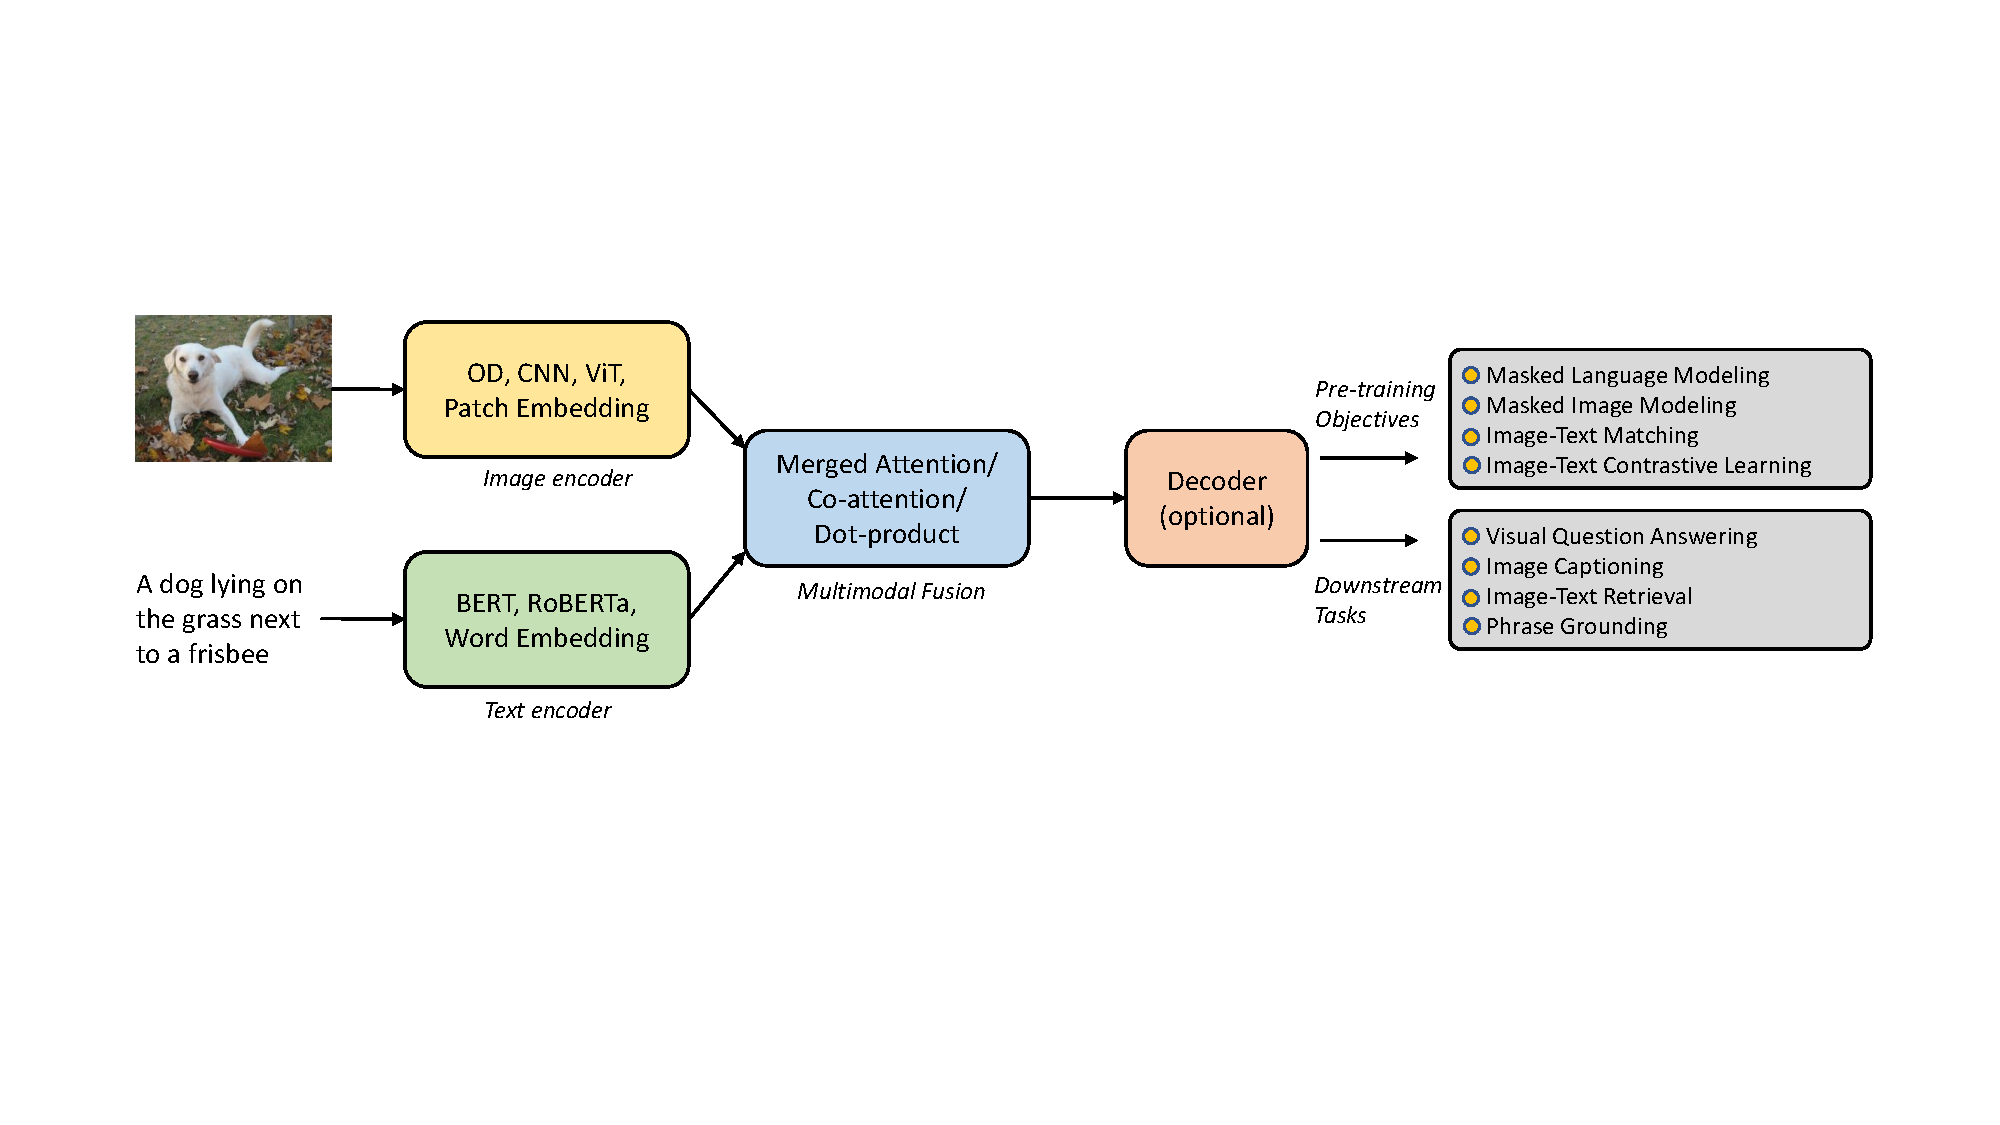
\includegraphics[width=\textwidth]{figures/multimodality/framework.pdf}
    \caption{ Illustration of a general framework for Transformer-based vision-language models.}
    \label{fig:framework}
\end{figure}

% \noindent \textbf{Overview}

A vision-language model typically consist of a \textit{text encoder}, a \textit{vision encoder}, a fusion module, and (optionally) a decoder.
Given an image-text pair, a VL model first extracts text features $w=\{w_1, \cdots, w_N\}$ and visual features $v=\{v_1, \cdots, v_M\}$ via a text encoder and a vision encoder, respectively. Here, $N$ is the number of tokens in a sentence, and $M$ is the number of visual features for an image, which can be the number of image regions/grids/patches, depending on the specific vision encoder being used.

The text and visual features are then fed into a \textit{multimodal fusion module} to produce cross-modal representations, which are then optionally fed into a \textit{decoder} before generating the final outputs. An illustration of this general framework is shown in Figure~\ref{fig:framework}.

In many cases, there are no clear boundaries among image/text backbones, multimodal fusion module, and the decoder. In this paper, we refer to the part of the model that only takes image/text features as input as the corresponding \emph{vision/text encoder}, and the part of the model that takes both image and text features as input as the \emph{multimodal fusion module}. Besides this, if there are additional modules that take the multimodal features as input to generate the output, we call it \emph{decoder}. We next describe different kinds of vision encoder, text encoder, and fusion module in detail.

\paragraph{Vision Encoder.} There are three types of vision encoders: ($i$) an object detector (OD), ($ii$) a plain CNN, and ($iii$) a vision Transformer. 
\begin{itemize}[leftmargin=*]
    \item \textbf{OD.} The most widely used object detector for VL research is the Faster R-CNN~\citep{ren2015faster} pre-trained on the Visual Genome (VG) dataset~\citep{krishna2016visual} as in BUTD~\citep{anderson2018bottom}. 
    In VinVL~\citep{zhang2021vinvl}, a stronger OD model based on the ResNeXt-152 C4 architecture is pre-trained on multiple public OD datasets (including COCO~\citep{chen2015microsoftcoco}, OpenImages~\citep{kuznetsova2020open}, Objects365~\citep{shao2019objects365} and VG), and significant performance boost is observed across a wide range of VL tasks by using this stronger OD model. Additional care is taken to encode the location information of image regions, which is typically represented as a 7-dimensional vector.\footnote{[$x_1,y_1,x_2,y_2,w,h,w*h$] (normalized top/left/bottom/right coordinates, width, height, and area)} Both visual and location features are then fed through a fully-connected layer, to be projected into the same embedding space. The final embedding for each region is obtained by summing up the two FC outputs and then passing through a layer normalization layer.
    %\mrinmaya{This makes it appear that every paper that uses objects does it this way. Can you provide a reference and explicitly state this as an example from that paper?}
    
    \item \textbf{CNN.} 
    In PixelBERT~\citep{huang2020pixel} and SOHO~\citep{huang2021seeing}, ResNet-50, ResNet-101 and ResNeXt-152 pre-trained from ImageNet classification are adopted. In CLIP-ViL~\citep{shen2021much}, ResNet-50, ResNet-101, and ResNet-50x4 pre-trained from CLIP~\citep{radford2021learning} are used. In SimVLM~\citep{wang2021simvlm}, they use the first three blocks (excluding the Conv stem) of ResNet-101 and ResNet-152 for their base and large models, respectively, and a larger variant of ResNet-152 with more channels for the huge model. Typically, it is observed that a stronger CNN backbone results in stronger downstream performance.
    \item \textbf{ViT.} Some recent pre-trained VLMs such as ALBEF~\citep{li2021align} and ViLT~\citep{kim2021vilt} use Transformer-based vision encoders. Following~\citet{dosovitskiy2020image}, an image is first split into image patches, which are then flattened into vectors and linearly projected to obtain patch embeddings. A learnable special token \texttt{[CLS]} embedding is also prepended to the sequence. These patch embeddings, when summed up together with learnable 1D position embeddings and a potential image-type embedding, are sent into a multi-layer Transformer block to obtain the final output image features.  
    Different ViT variants have been studied for VLP, such as plain ViT~\citep{dosovitskiy2020image}, DeiT~\citep{touvron2020deit}, BEiT~\citep{bao2021beit}, Swin Transformer~\citep{liu2021swin}, and  CLIP-ViT~\citep{radford2021learning}, to name a few.
\end{itemize}

In a nutshell, no matter what vision encoder is used, the input image is represented as a set of feature vectors $\vv=\{ \vv_1, \cdots, \vv_M\}$. VLMs can be categorized into non end-to-end models, which use an OD model to get vision features for the model, and end-to-end models that directly take raw images as input.



\paragraph{Text Encoder.} Following BERT~\citep{devlin-etal-2019-bert} and RoBERTa~\citep{liu2019roberta}, VLMs first segment the input sentence into a sequence of subwords and then insert two special tokens at the beginning and the end of the sentence to generate the input text sequence. After we obtain the text embeddings, existing works either feed them directly to the multimodal fusion module~\citep{li2019visualbert,chen2020uniter}, or to several text-specific layers~\citep{tan-bansal-2019-lxmert,lu2019vilbert} before the fusion. For the former, the fusion module is typically initialized with BERT, and the role of text encoding and multimodal fusion is therefore entangled and absorbed in a single BERT model, and in this case, we consider text encoder as the word embedding layer. 

In a nutshell, no matter what text encoder is used, the input text is represented as a set of feature vectors $w=\{ w_1, \cdots, w_N\}$.

\paragraph{Multimodal Fusion.} 
For \emph{dual encoders} like CLIP~\citep{radford2021learning} and ALIGN~\citep{jia2021scaling}, fusion is essentially computing the similarity between representation in the two modalities, which is typically performed via a dot-product between two global image and text feature vectors.
For \emph{fusion encoder}, it takes both $v=\{ v_1, \cdots, v_M\}$ and $w=\{ w_1, \cdots, w_N\}$ as input, and learns contextualized multimodal representations denoted as $\tilde{v}=\{ \tilde{v}_1, \cdots, \tilde{v}_M\}$ and $\tilde{w}=\{ \tilde{w}_1, \cdots, \tilde{w}_N\}$. There are mainly two types of fusion modules, namely, \textit{merged attention} and \textit{co-attention}, shown in Figure~\ref{fig:chp3_fusion}. Specifically,
\begin{itemize}[leftmargin=*]
    \item In a \textbf{merged attention} module, the text and visual features are simply concatenated together, and then fed into a single Transformer block. This design has been used in many previous works, such as VisualBERT~\citep{li2019visualbert}, Unicoder-VL~\citep{li2020unicoder}, VL-BERT~\citep{su2019vl}, UNITER~\citep{chen2020uniter}, OSCAR~\citep{li2020oscar}, VinVL~\citep{zhang2021vinvl}, ViLT~\citep{kim2021vilt}, GIT~\citep{wang2022git}, \emph{etc}. %\mrinmaya{Can we say more what we mean by merged atttention and co-attention mathematically. It would be helpful so that we can test students about this in the exam, etc.}
    \item In a \textbf{co-attention} module, on the other hand, the text and visual features are fed into different Transformer blocks independently, and techniques such as cross-attention are used to enable cross-modal interaction. This design has been used in LXMERT~\citep{tan-bansal-2019-lxmert}, ViLBERT~\citep{lu2019vilbert}, ERNIE-ViL~\citep{yu2021ernie}, METER~\citep{dou2021empirical}, \emph{etc}. Also, in many models, only image-to-text cross-attention modules are used, such as ALBEF~\citep{li2021align}, BLIP~\citep{li2022blip}, CoCa~\citep{yu2022coca}, and  Flamingo~\citep{alayrac2022flamingo}. Most ViT-based models adopts co-attention module since the image sequence can be very long and doing merged attention can be very computationally inefficient.
\end{itemize}



\begin{figure*}[t!]
  \centering
    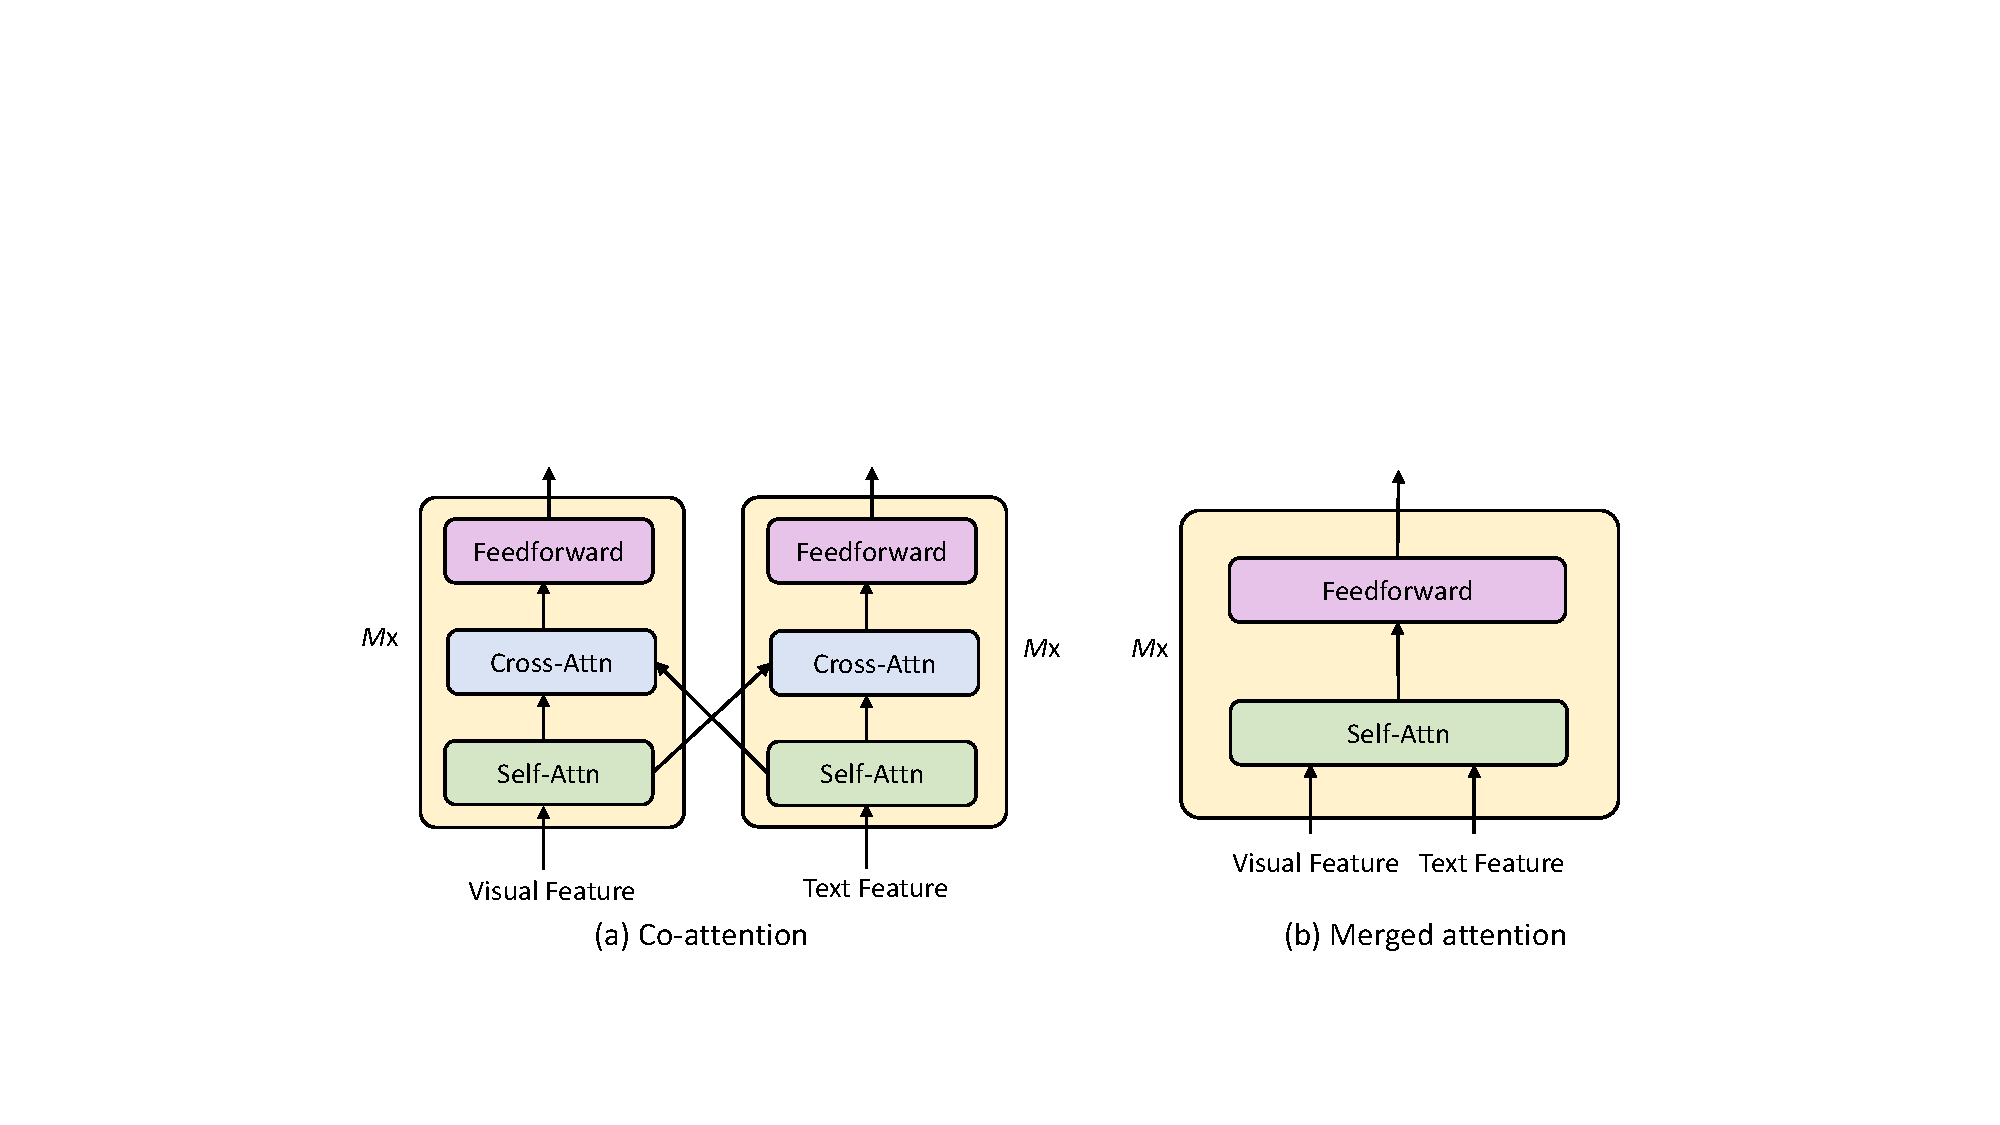
\includegraphics[width=0.8\linewidth]{figures/multimodality/fusion.pdf}
  \caption{Co-attention and merged attention design for multimodal fusion.}
  \label{fig:chp3_fusion}
  \vspace{-3mm}
\end{figure*}

\section{Vision-Language Models: Pre-training Objectives}

We then introduce the pre-training tasks used in VLP. We will first introduce masked language modeling and image-text matching, which have been used extensively in almost every VLP model. Then, we will also describe image-text contrastive learning and masked image modeling tasks which are widely used in recent VLMs. 

\paragraph{Masked Language Modeling (MLM).} 
The MLM objective is first introduced in language model pre-training~\citep[\textit{e.g.,}][]{devlin-etal-2019-bert,liu2019roberta}. In VLP, MLM with image-text pairs has also proven to be useful.
In MLM, given an image-text pair, we randomly mask out the input words with probability of 15\%, and replace the masked ones $\tilde{\mathbf{w}}_\mathbf{m}$ with special token \texttt{[MASK]}.\footnote{Following BERT, this 15\% is typically decomposed into 10\% random words, 10\% unchanged, and 80\% \texttt{[MASK]}.}
The goal is to predict these masked tokens based on their surrounding words $\tilde{\mathbf{w}}_{\setminus \mathbf{m}}$ and the paired image $\tilde{\mathbf{v}}$, by minimizing the negative log-likelihood:
\begin{equation}
    \mathcal{L}_{\text{MLM}}(\theta) = -\mathbb{E}_{(\tilde{\mathbf{w}}, \tilde{\mathbf{v}})\sim D} \log P_{\theta}(\tilde{\mathbf{w}}_\mathbf{m} | \tilde{\mathbf{w}}_{\setminus \mathbf{m}}, \tilde{\mathbf{v}})\,,
\end{equation}
where $\theta$ denotes the trainable parameters. 
Each pair $(\tilde{\mathbf{w}}, \tilde{\mathbf{v}})$ is sampled from the whole training set $D$. There are several MLM variants used in VLP. Specifically,
\begin{itemize}[leftmargin=*]
    \item \textbf{Seq-MLM}: In order to adapt the pre-trained model for image captioning, it is observed~\citep{zhou2020unified,wang2021ufo} that adding a seq2seq \emph{causal mask} during pre-training is beneficial. That is, in Seq-MLM, the model can only use its preceding context to predict the masked token, which is consistent to the way the model performs image captioning during inference.  
    \item \textbf{LM}: Direct language modeling is used in BLIP~\citep{li2022blip} and CoCa~\citep{yu2022coca} for VLP. The model predicts the caption given an image token-by-token autoregressively. 
    \item \textbf{Prefix-LM}: Using the encoder-decoder framework as in SimVLM~\citep{wang2021simvlm} and DaVinCi~\citep{diao2023write}, a PrefixLM pre-training objective is proposed, where a sentence is first split into two parts, and the bi-directional attention is enabled on the prefix sequence and the input image, while a causal attention mask is adopted on the remaining tokens. 
\end{itemize}

\paragraph{Image-Text Matching (ITM).} In ITM, given a batch of matched or mismatched image-caption pairs, the model needs to identify which images and captions correspond to each other. Most VLP models treat image-text matching as a binary classification problem. Specifically, a special token (\emph{i.e.}, $\texttt{[CLS]}$) is
appended at the beginning of the input sentence to learn a global cross-modal representation. We then feed the model with either a matched or mismatched image-caption pair $\langle \tilde{\mathbf{v}}, \tilde{\mathbf{w}} \rangle$ with equal probability, and a classifier is added on top of the $\texttt{[CLS]}$ token to predict
a binary label $y$, indicating whether the sampled image-caption pair is matched. Specifically, denote the output score as $s_{\theta}(\tilde{\mathbf{w}}, \tilde{\mathbf{v}})$, We apply the binary cross-entropy loss for optimization:
\begin{equation}
    \mathcal{L}_{\text{ITM}}(\theta) = - \mathbb{E}_{(\tilde{\mathbf{w}}, \tilde{\mathbf{v}})\sim D} [y \log s_{\theta}(\tilde{\mathbf{w}}, \tilde{\mathbf{v}}) + (1-y) \log (1-s_{\theta}(\tilde{\mathbf{w}}, \tilde{\mathbf{v}}))] )\,.
\end{equation}
Besides randomly sampling a negative image-text pair, harder negative pairs can also be mined from an image-text contrastive loss introduced below, which has been shown to be effective in improving the downstream performance, as reported in ALBEF~\citep{li2021align}, VLMo~\citep{wang2021vlmo}, and X-VLM~\citep{zeng2022x}. 

\paragraph{Image-Text Contrastive Learning (ITC).} Early VLP models, such as UNITER~\citep{chen2020uniter} and VinVL~\citep{zhang2021vinvl}, do not use ITC for pre-training. Though the ITC loss is widely studied before VLP, in the context of end-to-end VLP, it is mostly popularized by CLIP~\citep{radford2021learning} and ALIGN~\citep{jia2021scaling} to pre-train a dual encoder. Later on, it is also used to pre-train a fusion encoder as in ALBEF~\citep{li2021align}. Note that this ITC loss is used on top of the outputs of image and text encoders, before multimodal fusion (\emph{i.e.}, the use of $w$ and $v$, instead of $\tilde{w}$ and $\tilde{v}$). Specifically, given a batch of $N$ image-text pairs, ITC aims to predict the $N$ matched pairs from all the $N^2$ possible image-text pairs. With a little bit abuse of notation, let $\{v_i\}_{i=1}^N$ and $\{w_i\}_{i=1}^N$ denote respectively the normalized image vectors and text vectors in a training batch. To compute image-to-text and text-to-image similarities, we have: 
\begin{align}
    s_{i,j}^{i2t} = v_i^\top w_j, \,\, s_{i,j}^{t2i} = w_i^\top v_j \,,\\
    \mathcal{L}_{\text{ITC}}^{i2t}(\theta) = -\frac{1}{N} \sum_{i=1}^N\log\frac{\exp(s_{i,i}^{i2t}/\sigma)}{\sum_{j=1}^N \exp (s_{i,j}^{i2t}/\sigma)} \,,\\ \mathcal{L}_{\text{ITC}}^{t2i}(\theta) = -\frac{1}{N} \sum_{i=1}^N\log\frac{\exp(s_{i,i}^{t2i}/\sigma)}{\sum_{j=1}^N \exp (s_{i,j}^{t2i}/\sigma)}\,,
\end{align}
where $\sigma$ is a learned temperature hyper-parameter,  $\mathcal{L}_{\text{ITC}}^{i2t}$ and $\mathcal{L}_{\text{ITC}}^{t2i}$ are image-to-text and text-to-image contrastive loss, respectively.

\paragraph{Masked Image Modeling (MIM).} Similar to the MLM objective, researchers have studied various masked image modeling (MIM) tasks for pre-training. Specifically, the model is trained to reconstruct the masked patches or regions $\tilde{\mathbf{v}}_{\mathbf{m}}$ given the remaining visible patches or regions $\tilde{\mathbf{v}}_{\setminus \mathbf{m}}$ and all the words $\tilde{\mathbf{w}}$ as 
\begin{equation}
    \mathcal{L}_{\text{MIM}}(\theta) = \mathbb{E}_{(\tilde{\mathbf{w}}, \tilde{\mathbf{v}})\sim D} P_{\theta}(\tilde{\mathbf{v}}_\mathbf{m} | \tilde{\mathbf{v}}_{\setminus \mathbf{m}}, \tilde{\mathbf{w}})\,.
\end{equation}
The designs of MIM can be divided into two categories.
\begin{itemize}[leftmargin=*]
    \item \textbf{For OD-based VLP models}, \emph{e.g.}, LXMERT~\citep{tan-bansal-2019-lxmert} and UNITER~\citep{chen2020uniter}, some of the input regions are randomly masked (\emph{i.e.}, the visual features of the masked regions are replaced by zeros), and the model is trained to regress the original region features via minimizing the mean squared error loss. Researchers~\citep{tan-bansal-2019-lxmert,lu2019vilbert,chen2020uniter} have also tried to first generate object labels for each region using a pre-trained object detector, which can contain high-level semantic information, and the model is trained to predict the object labels for the masked regions instead of the original region features. 
    \item \textbf{For end-to-end VLP models}, \emph{e.g.}, ViLT~\citep{kim2021vilt} and METER~\citep{dou2021empirical}, researchers have investigated the use of masked patch regression/classification for masked image modeling. Specifically, 
        \begin{itemize}[leftmargin=*]
            \item For \textbf{MIM with discrete VQ tokens}, inspired by BEiT~\citep{bao2021beit}, discrete VQ tokens are first extracted for the input patches, and the model is then trained to reconstruct the discrete tokens. Specifically, the VQ-VAE~\citep{van2017neural} model in DALL-E~\citep{ramesh2021dalle} is first used to tokenize each image into a sequence of discrete tokens. Each image is resized so that the number of patches is equal to the number of tokens, and thus each patch corresponds to a discrete token. Then, we randomly mask 15\% of the patches and feed the masked image patches to the model as before, but now the model is trained to predict the discrete tokens instead of the masked patches.
            \item For \textbf{MIM with in-batch negatives}, by imitating MLM which uses a text vocabulary, the model is trained to reconstruct input patches by using a dynamical vocabulary constructed with in-batch negatives. Concretely, at each training step, we sample a batch of image-caption pairs $\{ \langle v^k, w^k \rangle \}_{k=1}^B$, where $B$ is the batch size. We treat all the patches in $\{ \mathbf{v}^k \}_{k=1}^B$ as candidate patches. For each masked patch, we mask 15\% of the input patches. The model needs to select the original patch within this candidate set. The model is trained to maximize its probability similar to noise contrastive estimation~\citep{nce1}.
        \end{itemize}
\end{itemize}

Notably, recent state-of-the-art VLP models (\emph{e.g.}, VinVL~\citep{zhang2021vinvl}, ALBEF~\citep{li2021align}, VLMo~\citep{wang2021vlmo}) do not apply MIM during pre-training, and in ViLT~\citep{kim2021vilt} and METER~\citep{dou2021empirical}, the authors also demonstrate that MIM is not helpful for downstream performance. However, there are also recent works that adopt masked vision-language modeling (as in MaskVLM~\citep{kwon2022masked} and VL-BEiT~\citep{bao2022vl}), which try to randomly mask patches/tokens while keeping the other modality intact.


